\documentclass{beamer}

\usepackage{presentation}

\title{Adversarial Attacks Against Medical Deep Learning Systems}
\date{June 27, 2018}
\author{James Campbell}
\institute{Cardiff University, School of Mathematics}

\begin{document}
\maketitle


\section{Deep Learning in Medicine}

\begin{frame}{Deep Learning in Medicine}
\centering
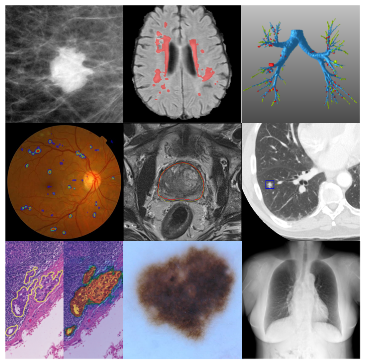
\includegraphics[width=0.6\textwidth]{./images/medical-deep-learning.png}

\cite{Litjens_Kooi_Bejnordi_Setio_Ciompi_Ghafoorian_van_der_Laak_van_Ginneken_Sánchez_2017}
\end{frame}

\begin{frame}{Deep Learning in Medicine}
\centering

\includegraphics[width=0.7\textwidth]{./images/fda.png}

\cite{Commissioner}
\end{frame}


\section{Adversarial Attacks}

\begin{frame}{Adversarial Attacks}
\centering
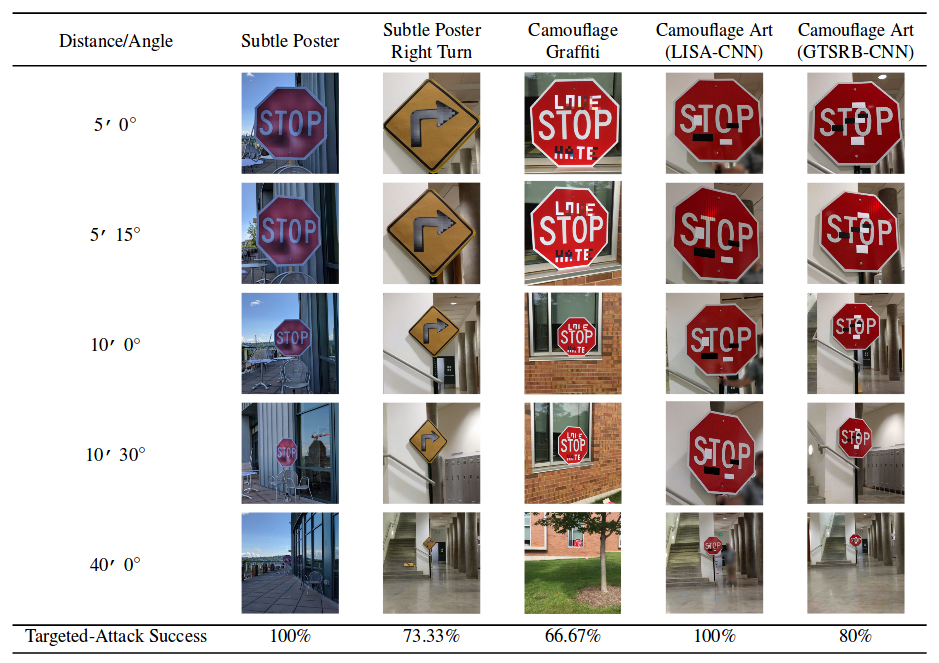
\includegraphics[width=0.9\textwidth]{./images/adverse-road-sign.png}

\cite{Eykholt_Evtimov_Fernandes_Li_Rahmati_Xiao_Prakash_Kohno_Song_2017}
\end{frame}


\begin{frame}{Adversarial Attacks}
Fool Google's InceptionV3 image classifier \href{https://www.youtube.com/watch?v=piYnd_wYlT8}{\alert{video}}.
\cite{Athalye_Engstrom_Ilyas_Kwok_2017, Ilyas_Engstrom_Athalye_Lin_2018}
\end{frame}



\section{Why Medicine?}

\begin{frame}{Why is Medicine important?}
\begin{itemize}
    \item An incorrect diagnosis can be dangerous to patients
    \pause
    \item Healthcare economy is huge and fraud is already a major problem \cite{Jain_Nundy_Abbasi_2014}
    \pause
    \item Increasing use in clinical trials \cite{Pien_Fischman_Thrall_Sorensen_2005}
\end{itemize}
\end{frame}

\begin{frame}{Why is Medicine particularly susceptible?}
\begin{itemize}
    \item Ambiguous ground truth \cite{Njeh_2008}
    \pause
    \item Images are standardised
    \pause
    \item Popular Architectures are often used
    \pause
    \item Many potential adversaries
\end{itemize}

\end{frame}

\section{Current Research}

\begin{frame}{Fast Gradient Sign Method}
Let $\theta$ be the parameters of a model, $x$ an input to the model and $y$ the target associated with $x$.
We also have a well defined loss function $L(\theta, x, y)$.

\pause

Then FGSM computes an adversarial example as:
$$
x + \epsilon \cdot \text{sign}( \nabla_{x} L(\theta, x, y))
$$

\cite{Goodfellow_Shlens_Szegedy_2014}
\end{frame}

\begin{frame}{Projected Gradient Descent}
PGD make this an iterative process.
We specify a set of allowed perturbations $\mathcal{S} \in \mathbb{R}^{d}$ (commonly the $l_{\infty}$ ball around $x$) and compute:
\pause

$$
x^{t+1} = \Pi_{x + \mathcal{S}} (x^{t} + \epsilon \cdot \text{sign}(\nabla_{x} L(\theta, x, y)))
$$

\cite{Madry_Makelov_Schmidt_Tsipras_Vladu_2017}
\end{frame}


\begin{frame}{Small Issue}
What if we don't have access to the model?
\pause

\begin{itemize}
    \item If we know the architecture, train our own version
    \pause
    \item If we don't know the architecture, but have access to probabilities, use NES (Natural Evolutionary Strategies) Gradient Estimate \cite{Ilyas_Engstrom_Athalye_Lin_2018}
    \pause
    \item If we only have access to predicted class, use a Monte Carlo approximation \cite{Ilyas_Engstrom_Athalye_Lin_2018}
\end{itemize}
\end{frame}

\begin{frame}{Current Research}
Hello, world! \cite{Finlayson_Chung_Kohane_Beam_2018}
\end{frame}

\section{Our Plan}

\begin{frame}{Our Plan}
\begin{itemize}
    \item Break the best deep learning systems
    \pause
    \item Understand how they were broken
    \pause
    \item Make them more robust
\end{itemize}
\end{frame}



\begin{frame}[allowframebreaks]{References}
    \printbibliography
\end{frame}


\end{document}
